\section{Priority Queues}
In this section we will discuss \textbf{min-heaps} which will help us sort
maintain elements in a sorted data structure.

\begin{Def}[Balanced Tree]

    A \textbf{balanced tree} is a tree where the height of the left and right subtrees of every node differ by at most one.
\end{Def}

\begin{Tip}
    To spot this, observe each level of the tree and see whether after consecutive levels, one branch has more nodes than the other.
\end{Tip}
\newpage
\noindent
Below is an example of a balanced tree and an unbalanced tree:
\begin{figure}[h!]
    \centering
    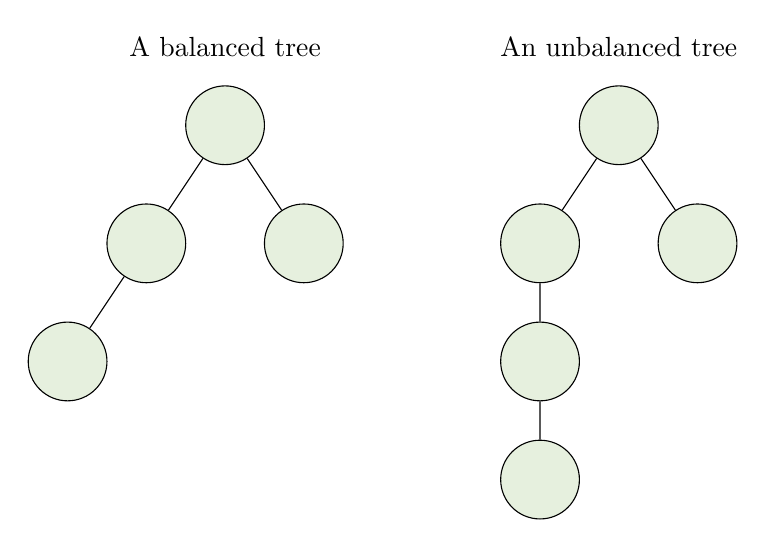
\begin{tikzpicture}[
        node/.style={circle, draw, fill=OliveGreen!10, minimum size=1cm},
        level distance=1.5cm,
        sibling distance=2cm
    ]

    % Left tree: height balanced
    \node[node] {}
        child {node[node] {}
            child {node[node] {}}
            child[missing]}
        child {node[node] {}};

    \node at (0, 1) {A balanced tree};

    % Right tree: not height balanced
    \node[node] at (5, 0) {}
        child {node[node] {}
            child {node[node] {}
            child {node[node] {}}}}
        child {node[node] {}};
            

    \node at (5, 1) {An unbalanced tree};

    \end{tikzpicture}
    \caption{Examples of a balanced tree and an unbalanced tree}
    \label{fig:balanced_unbalanced_trees}
\end{figure}
\begin{Def}[Binary Search Tree]

    A \textbf{binary tree} is a where each parent node $p_i$ has at most two children $c_{left}$ and $c_{right}$.\\
    A \textbf{binary search tree} has each child ($c_{left} > \text{p}_{i}$) and ($c_{right} < \text{p}_{i}$).\\

    \noindent
    With $n$ nodes, there are $n-1$ edges.
\end{Def}

\begin{Def}[Heap]

    A \textbf{heap} is a binary tree with the following properties:
    \begin{enumerate}
        \item[(i.)] It is a \textbf{complete binary tree} (a binary and balanced tree).
        \item[(ii.)] It is a \textbf{min-heap} if the parent node is less than its children.
        \item[(iii.)] It is a \textbf{max-heap} if the parent node is greater than its children.
    \end{enumerate}
    \noindent
    \textbf{Operations:} Suppose we have a heap of $n$ elements:
    \begin{itemize}
        \item \textbf{PEEK:} Return the root. $O(1)$;
        \item \textbf{INSERT:} Add a new element. $log(n)$;
        \item \textbf{EXTRACT:} Remove the root. $log(n)$;
        \item \textbf{UPDATE:} Update an element. $log(n)$;
    \end{itemize}
\end{Def}

\newpage

\begin{Tip}
    The difference between a min-heap and a binary search tree, is that $c_{left} \leq c_{right} \leq \text{p}_{i}$. That is, the left and right child in a min-heap are not ordered, just less than the parent;
    Contrary to a binary search tree where the left child is less than the parent and the right child is greater.
\end{Tip}

\noindent 
We use a min-heap as a data structure to maintain a sorted list as an input.

\begin{Func}[find\_compatible\_room - \texttt{FCR($c$, $A$, $Q$)}]
    Finds a compatible room for class $c$ based on the current room schedule.

    \vspace{.5em}
    \noindent
    \textbf{Input:} Class ID $c$, current schedule $A$, priority queue $Q$ with room finish times.\\
    \textbf{Output:} The room $k$ compatible with class $c$ or \texttt{None}.\\
    \begin{algorithm}[H]
        \SetAlgoLined
        \tcp{$c$: class id, $A$: current schedule of room assignments}
        \tcp{$Q$: priority queue with room finish times}
        $\langle f_k, k \rangle \gets \text{PEEK\_MIN}(Q)$ \tcp*[f]{shows lowest $\langle$key, value$\rangle$ pair, $O(1)$}

        \If{$s_c > f_k$ \tcp*[f]{finish time in room $k$}}{
            \KwRet{$k$} \tcp*[f]{$c$ is compatible with room $k$}
        }
        \Else{
            \KwRet{\texttt{None}}\;
        }
    \end{algorithm}

    \noindent
    \textbf{Time Complexity:} $O(n)$ as now we only need to check the minimum finish time in the priority queue.\\
    \textbf{Space Complexity:} $O(n+m)$ if our min-heap is implemented as a hash table.
\end{Func}

\noindent
We can also implement a min-heap for sorting classes as well. 
\newpage
\begin{Func}[EarliestStartTimeFirst Algorithm - \texttt{EarliestStartTimeFirst($j = 1 \dots n : s_j, f_j$)}]
    Finds an optimal schedule of lectures based on their earliest start time.

    \vspace{.5em}
    \noindent
    \textbf{Input:} Start times $s_j$ and finish times $f_j$ of classes.\\
    \textbf{Output:} Assignment of lectures to rooms.\\
    \begin{algorithm}[H]
        \SetAlgoLined
        \tcp{$s_j, f_j$: start and finish times of classes}
        $\mathcal{A} \gets$ empty hash table \tcp*[f]{$\mathcal{A}[k]$ contains the list of courses assigned to room $k$}
        $Q \gets$ empty priority queue \tcp*[f]{contains $\langle$finishTime, roomId$\rangle$ pairs}
        sorted\_class $\gets$ sort($s_1, \dots, s_n$) \tcp*[f]{sort by start time}
        
        \For{each $c$ in sorted\_class}{
            $k \gets$ find\_compatible\_room($c$, $\mathcal{A}$, $Q$)\;
            \If{$k$ is not None}{
                $\mathcal{A}[k]$.add($c$)\;
                $Q$.UPDATE-KEY($\langle f_k, k \rangle, \langle f_c, k \rangle$) \tcp*[f]{update finish time of room $k$}
            }
            \Else{
                $d \gets$ len($\mathcal{A}$) \tcp*[f]{highest room id}
                $\mathcal{A}[d + 1] \gets [\ ]$ \tcp*[f]{open new room}
                $\mathcal{A}[d + 1]$.add($c$)\;
                $Q$.INSERT($\langle f_c, d + 1 \rangle$)\;
            }
        }
        \KwRet{$\mathcal{A}$}
    \end{algorithm}

    \noindent
    \textbf{Time Complexity:} $O(n\log n)$ as inserting into a min heap is $O(\log n)$ and reading is $O(1)$.\\
    \textbf{Space Complexity:} $O(n)$ storing the input of $n$ classes.
\end{Func}

\begin{theo}[Heap Array Representation]

    A heap $H$ can be represented by a zero-indexed array $A$ via:
    \begin{itemize}
        \item[(i.)] The root is at index $0$.
        \item[(ii.)] The left child of node $i$ is at index $2i + 1$.
        \item[(iii.)] The right child of node $i$ is at index $2i + 2$.
    \end{itemize}

    \noindent
    Enabling a \textbf{space complexity} of $O(n)$.
\end{theo}
\newpage


